\documentclass[tikz,border=10pt, dvipsnames]{standalone}
\usepackage{tikz}
\usetikzlibrary{positioning, shapes, arrows, bending}

\begin{document}
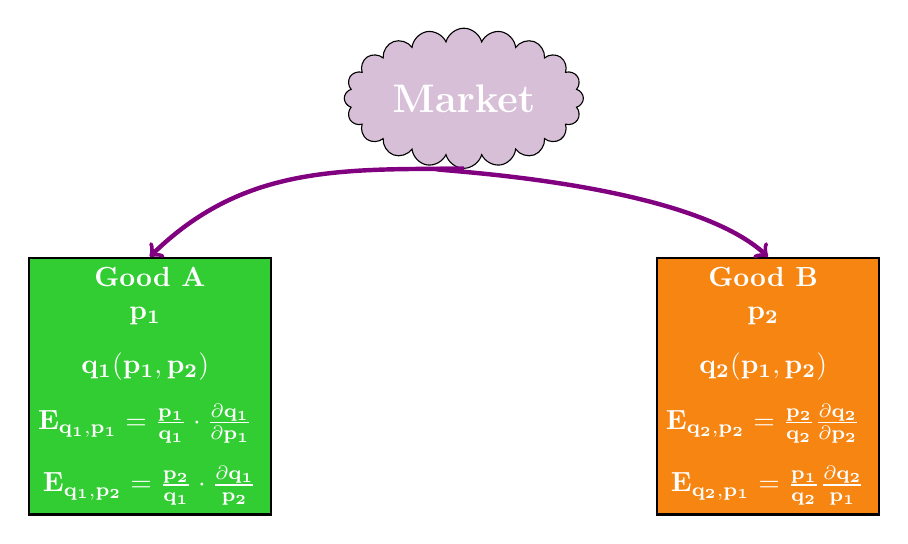
\begin{tikzpicture}[node distance=20mm]
\node[draw, cloud, cloud puffs = 20, aspect = 2, fill = Thistle] (A) at (current page.center) {\Large\textbf{\textcolor{white}{Market}}};
\node[draw, thick, rectangle, below left=of A, align = center, fill = LimeGreen] (B) {
\textbf{\textcolor{white}{Good A}} \\ 
$\color{white} \mathbf{p_{1}}$  \vspace{0.2 cm}\\  
$\color{white} \mathbf{q_{1}(p_{1}, p_{2})}$ \vspace{0.2 cm} \\
$\color{white}\mathbf{ E_{q_{1}, p_{1}} = \frac{p_{1}}{q_{1}} \cdot \frac{\partial q_{1}}{\partial p_{1}}}$ \vspace{0.2 cm }\\
$\color{white} \mathbf{E_{q_{1}, p_{2}} = \frac{p_{2}}{q_{1}} \cdot \frac{\partial q_{1}}{p_{2}}}$
};
\node[draw,thick, rectangle, below right=of A, align = center, fill = BurntOrange] (C) {
\textbf{\textcolor{white}{Good B}} \vspace{0.2 cm} \\
$\color{white} \mathbf{p_{2}}$ \vspace{0.2 cm} \\
$\color{white} \mathbf{q_{2}(p_{1}, p_{2})}$ \vspace{0.2 cm} \\
$\color{white} \mathbf{E_{q_{2}, p_{2}} = \frac{p_{2}}{q_{2}}\frac{\partial q_{2}}{\partial p_{2}}}$ \vspace{0.2 cm} \\
$\color{white} \mathbf{E_{q_{2}, p_{1}} = \frac{p_{1}}{q_{2}} \frac{\partial q_{2}}{p_{1}}}$
};
\draw[->, ultra thick, violet] (A.south) to [out = 180, in = 45] (B.north); 
\draw[->, ultra thick, violet] (A.south) to [out = 180, in = 135] (C.north); 
\end{tikzpicture}
\end{document}